% ===== s07_ablation =====
\section{Ablation Study}
The ablation replaces the 42 input columns of the compact MLP with the three highest-ranked genuine traffic features (\texttt{orig\_ip\_bytes}, \texttt{duration}, \texttt{orig\_pkts}) while keeping all other settings unchanged (Table~\ref{tab:abl}, Fig.~\ref{fig:abl}).

\begin{table}[!t]
\centering
\caption{Ablation of the compact MLP (single run, seed 42).}
\label{tab:abl}
\footnotesize
\begin{tabular}{@{}lccc@{}}
\toprule
\textbf{Metric} & \textbf{42 features} & \textbf{Top-3 features} & \textbf{Change} \\
\midrule
Parameters & 4,865 & 2,369 & $-51.3\%$ \\
Macro-F1 & 0.6904 & 0.6796 & $-0.0108$ \\
ROC-AUC & 0.7135 & 0.6401 & $-0.0734$ \\
FPR & 0.6115 & 0.6330 & $+0.0215$ \\
Final training loss & 0.4868 & 0.5218 & $+0.0350$ \\
\bottomrule
\end{tabular}
\end{table}

\begin{figure}[!t]
\centering
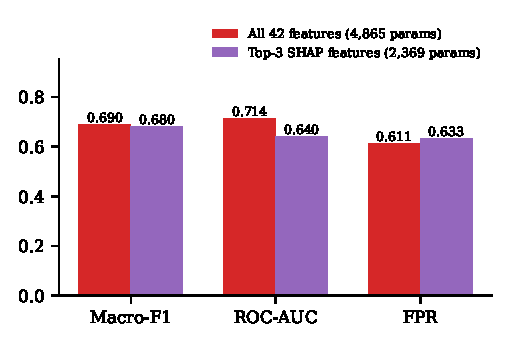
\includegraphics[width=0.85\columnwidth]{figures/fig_ablation.pdf}
\caption{Effect of reducing the compact MLP to the top-3 SHAP traffic features.}
\label{fig:abl}
\end{figure}

Reducing the input to three features cut the parameter count by 51.3\% but lowered ROC-AUC by 0.0734 and raised the FPR slightly, so the three features do not carry enough of the signal for this MLP. The macro-F1 change is small (0.0108) because both models already predict most flows as attacks. Other components (SMOTE, scaling, dropout, and the choice of explainer model) were not ablated, so their contributions are unknown.